############ OLD INTRO ############

Los juegos de lógica o estrategia han sido utilizados como {\it benchmark} en los inicios del campo de la inteligencia artificial. Pese a que principalmente se han utilizado juegos de mesa o de cartas dadas las facilidades a la hora de representar su modelo, con el avance de la tecnología y la llegada de los videojuegos en ordenador existe la posibilidad de que los mismos puedan ser una nueva herramienta con la que experimentar y explorar diferentes técnicas e implementaciones de IA. En la actualidad prácticamente todos los videojuegos que incorporan elementos que simulan comportamiento humano lo hacen con lógica determinista y patrones definidos, sin incorporar ningún tipo de simulación de pensamiento complejo. Algunas de las razones causantes de este fenómeno son:

\begin{itemize}
{\item La diferencia en la dificultad de implementación entre patrones simples y un agente complejo.}
{\item El hecho de que un agente puede llegar a ser demasiado efectivo a la hora de competir contra un humano.}
{\item Limitaciones en la capacidad de computación restante cuando el sistema está ejecutando un videojuego ya que suelen ser aplicaciones significativamente pesadas y complejas.}
\end{itemize}


Sin embargo, estos problemas son solventables y debemos tener en cuenta los beneficios que se pueden obtener al trabajar con videojuegos reales. En la actualidad, somos capaces de simular grandes mundos con millones de entidades y jugadores reales. En muchas ocasiones los entornos presentados son capaces de representar simulaciones muy precisas de como se comporta el mundo real. Esto puede darse en varios sentidos, un buen ejemplo son los videojuegos basados en físicas que permiten observar como objetos e individuos interactúan entre ellos siguiendo leyes de la física que se ajustan con mucha precisión a las reales. En otros casos se pueden simular verdaderas comunidades de gente real en videojuegos del genero MMO\footnote{Massively Multiplayer Online: Videojuegos que reúnen a cantidades enormes de jugadores en el mismo mundo y conectados en línea.} por lo que se puede obtener de los mismos datos de comportamientos reales sin necesidad de lidiar con las dificultades de obtenerlos del mundo real.

\bigskip

Por estas razones se podría considerar que un videojuego está mucho mas cerca de ser capaz de modelar el mundo real que un juego de mesa, lo que lo hace un banco de trabajo adecuado para investigar y experimentar con Inteligencia Artificial. Técnicas como redes neuronales, computación evolutiva o lógica difusa pueden funcionar en situaciones en tiempo real, continuas y complejas que presentan tanto nuestra realidad como los videojuegos. Pese a esto, actualmente en muy pocas ocasiones se experimenta con técnicas de IA utilizando videojuegos.

\bigskip

Por esto se pretende implementar un videojuego con la necesidad de incorporar un competidor que requiera ser controlado por la propia aplicación. Una vez creado el videojuego se agregarán los elementos necesarios relacionados con el campo de la inteligencia artificial. Para ello se implementará un agente que compita con un jugador real. Ambos se moverán libremente en un espacio de posiciones continuo. Además realizarán una serie de acciones ofensivas y defensivas con el objetivo de derrotar a su oponente.

\bigskip

Con este fin, se pretende realizar una implementación de un juego que permita al agente tener acceso a los estados en los que se encuentran él y su competidor así como las acciones que puede realizar en un determinado momento. Se buscará un competidor no solo apto pero también justo. Además, esto nos permitirá realizar un entrenamiento en el que el propio agente podrá competir con él mismo para aprender los fundamentos del juego además de competir contra jugadores humanos u otras implementaciones tradicionales. Esto nos brinda la posibilidad de determinar como reacciona ante estos y si es capaz de adaptarse a los posiblemente distintos estilos de juego contra los que se tendrá que enfrentar.






###### intro #####


\bigskip

La materialización de uno de los riesgos del proyecto descrito en el apartado \ref{AC} ha tenido un impacto relevante sobre la complejidad y completitud del agente. La primera aproximación al trabajo implicaba utilizar una demostración de la aplicación del videojuego realizada en un motor conocido pero surgió la necesidad de implementar la aplicación desde cero.

\bigskip

No existe una suficiente variedad de herramientas para trabajar con técnicas de inteligencia artificial en videojuegos, solo un grupo pequeño de competiciones y videojuegos ya sobre-explotados.



###### UNITY ######

\section{Prototipo de Unity}

Dado que el prototipo inicial realizado en Unity ha tenido un impacto significativo en el proyecto, tal y como se muestra en la sección \ref{AC}, se dedica este subapartado a mostrar los problemas que ha generado el elegir esta tecnología como primera opción.

\bigskip

En las figuras \ref{unity:combate} y \ref{unity:limite} podemos observar dos capturas del prototipo. En ambos casos se observan las vallas pensadas para limitar el área de combate. Las mismas cuentan con atributos que hacen que generen colisiones, es decir, que los personajes no puedan atravesarlas en ningún caso.

\bigskip

Sin embargo, al escalar el tiempo por valores relativamente pequeños, este tipo de funcionalidades dejan de funcionar ya que el motor tarda demasiado en componer cada uno de los fotogramas, haciendo que en muchas ocasiones en un fotograma se calcule que el personaje está en un lado de la valla y en el siguiente esté en el otro sin haber entrado en contacto con la misma.

\bigskip

Este tipo de fallos son inaceptables ya que rompen el funcionamiento de las mecánicas de juego al realizar las simulaciones, haciendo que un posible agente no pudiera aprender de forma eficaz y eficiente.

\bigskip

Algo parecido sucede con los ataques. Al intentar acelerar el tiempo y realizar un ataque ocurre con cierta frecuencia que el motor se salta los fotogramas en los que realmente se está comprobando si se hace daño al enemigo, inutilizando esta mecánica también.

\bigskip

En aras de permitir una visualización más comprensible de los problemas se pone a disposición un vídeo en \textit{YouTube}\footnote{disponible en: \url{https://youtu.be/PY4H8dk8zcU}} en el que se muestra concretamente el problema de la valla. Es cierto que en este caso sí se está mostrando la aplicación y no se está eliminando la visualización para aumentar el rendimiento, sin embargo se ha comprobado que los problemas son los mismos incluso sin visualización. Además el tiempo solo está escalado 20 veces, lo que se esperaría que fuera soportable para el motor pero no es así. Como comparación, en el producto final se escala unas 600 veces sin problema alguno.

\begin{figure}
	\centerline{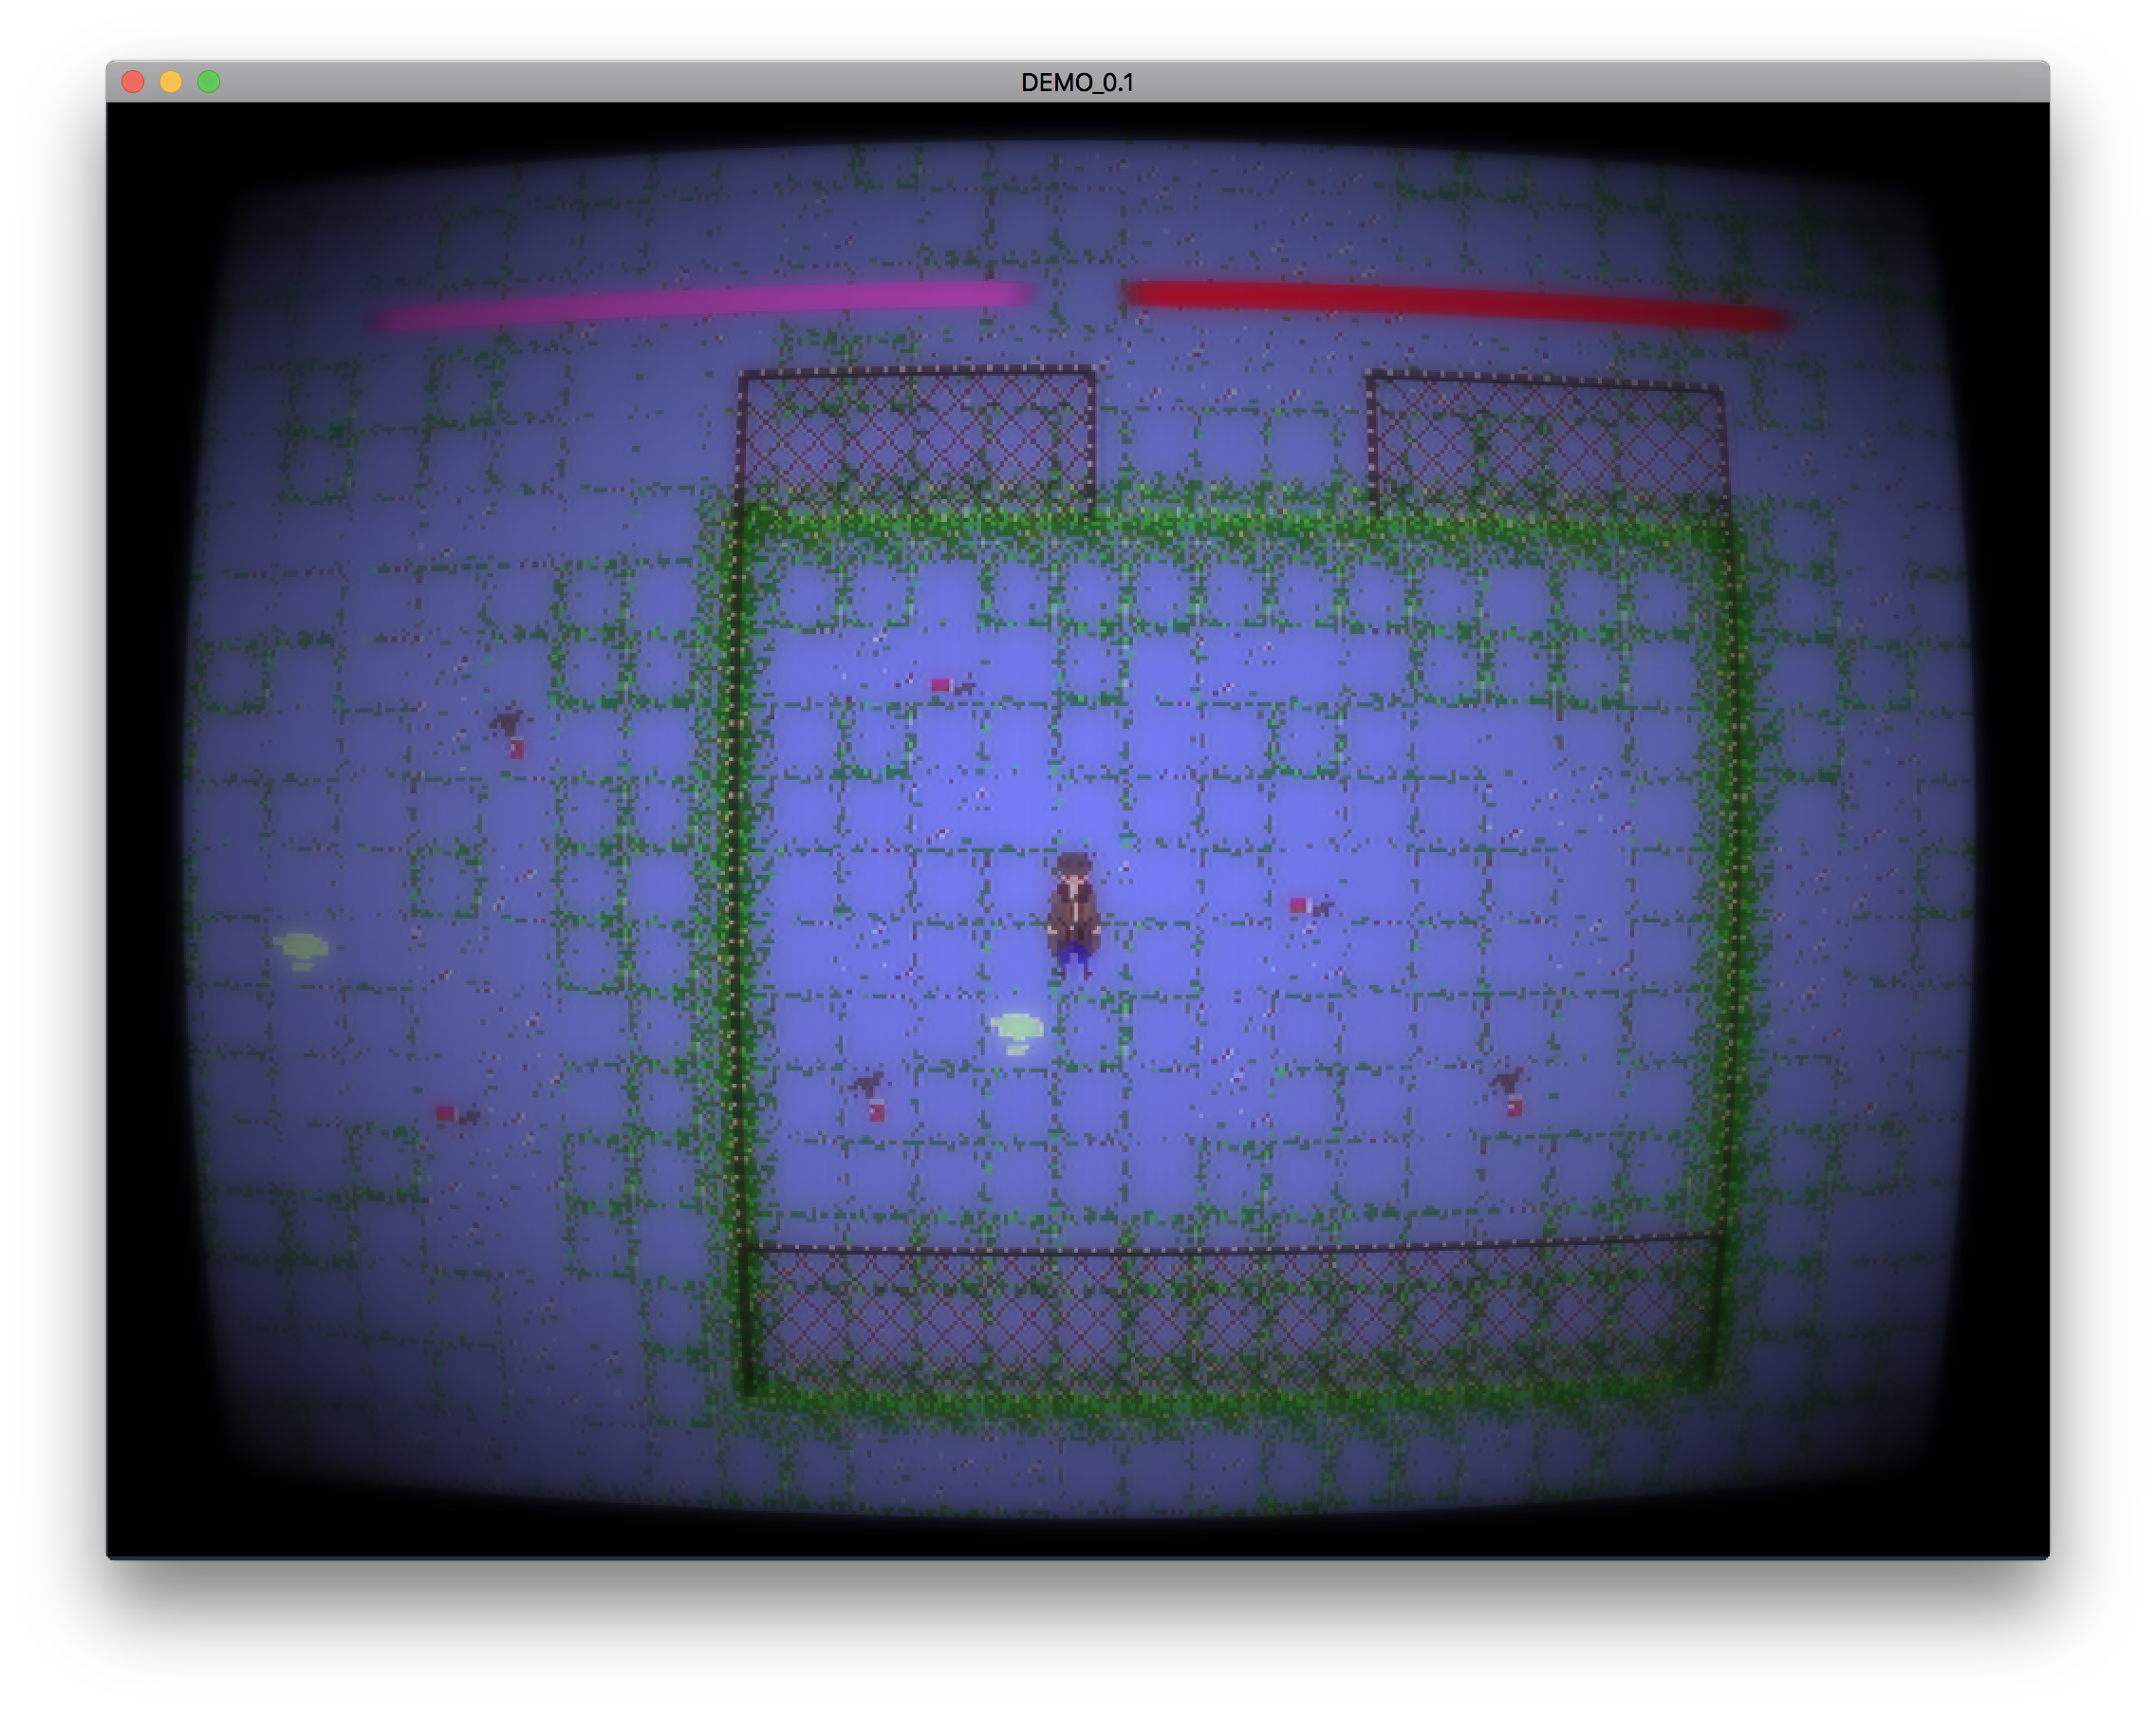
\includegraphics[width=15cm]{otros/otrasCapturas/valla1.png}}
	\caption{Captura del prototipo en la zona de combate}
	\label{unity:combate}
\end{figure}

\begin{figure}
	\centerline{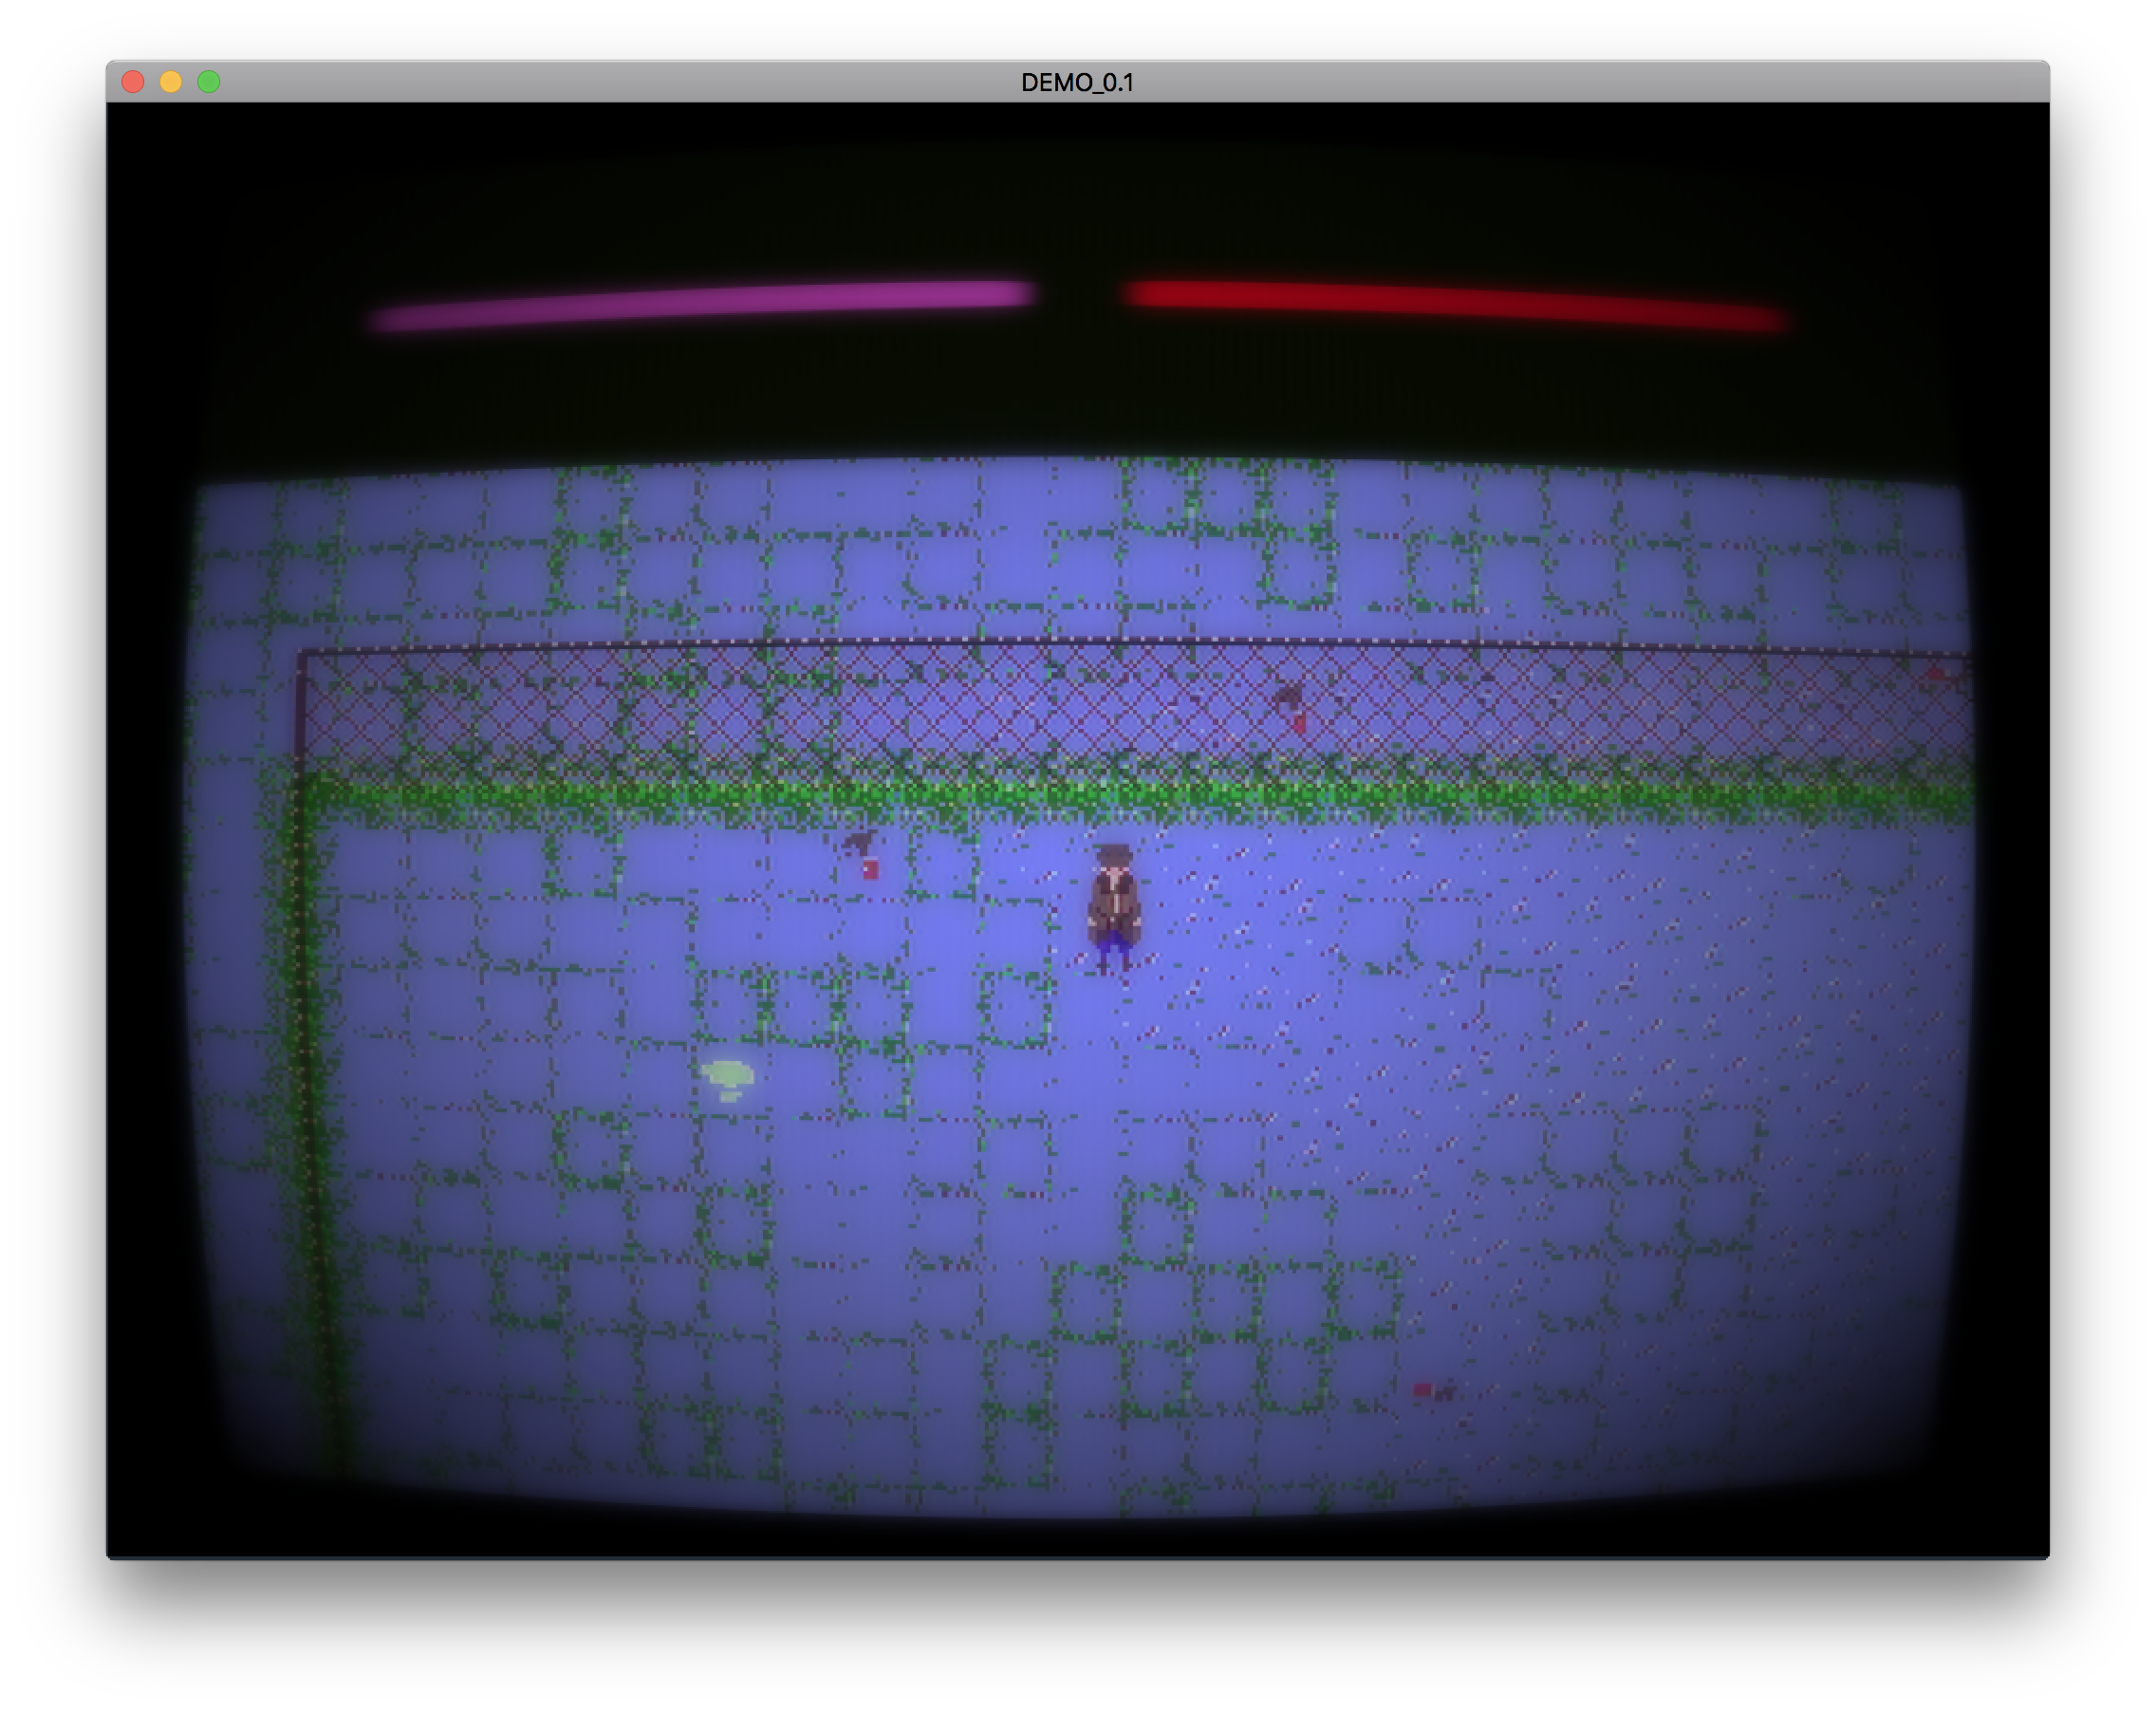
\includegraphics[width=15cm]{otros/otrasCapturas/valla2.png}}
	\caption{Captura del prototipo en el límite del mapa}
	\label{unity:limite}
\end{figure}
